\documentclass[10pt,letterpaper]{article}
\usepackage[utf8x]{inputenc}
\usepackage{ucs}
\usepackage[spanish]{babel}
\usepackage{amsmath}
\usepackage{amsfonts}
\usepackage{amssymb}
\usepackage{graphicx}
\sloppy
\setlength{\parindent}{0pt}
\usepackage[none]{hyphenat}
\usepackage[left=0.5cm,right=0.5cm,top=0.5cm,bottom=0.5cm]{geometry}
\author{F\'elix Ernesto Charry Pastrana}
\begin{document}
\textbf{Universidad Nacional Autónoma de México}\\
Presentado a: \textbf{Santiago Caballero}\\ 
Presentado por: \textbf{F. E. Charry-Pastrana}\\
Maestría en Ciencias Físicas \\
Introducción a la física computacional \\
Mayo de 2018 \\
\begin{center}
\textbf{\begin{LARGE}
Péndulo doble
\end{LARGE}}
\end{center}
\begin{figure}[h]
\centering 
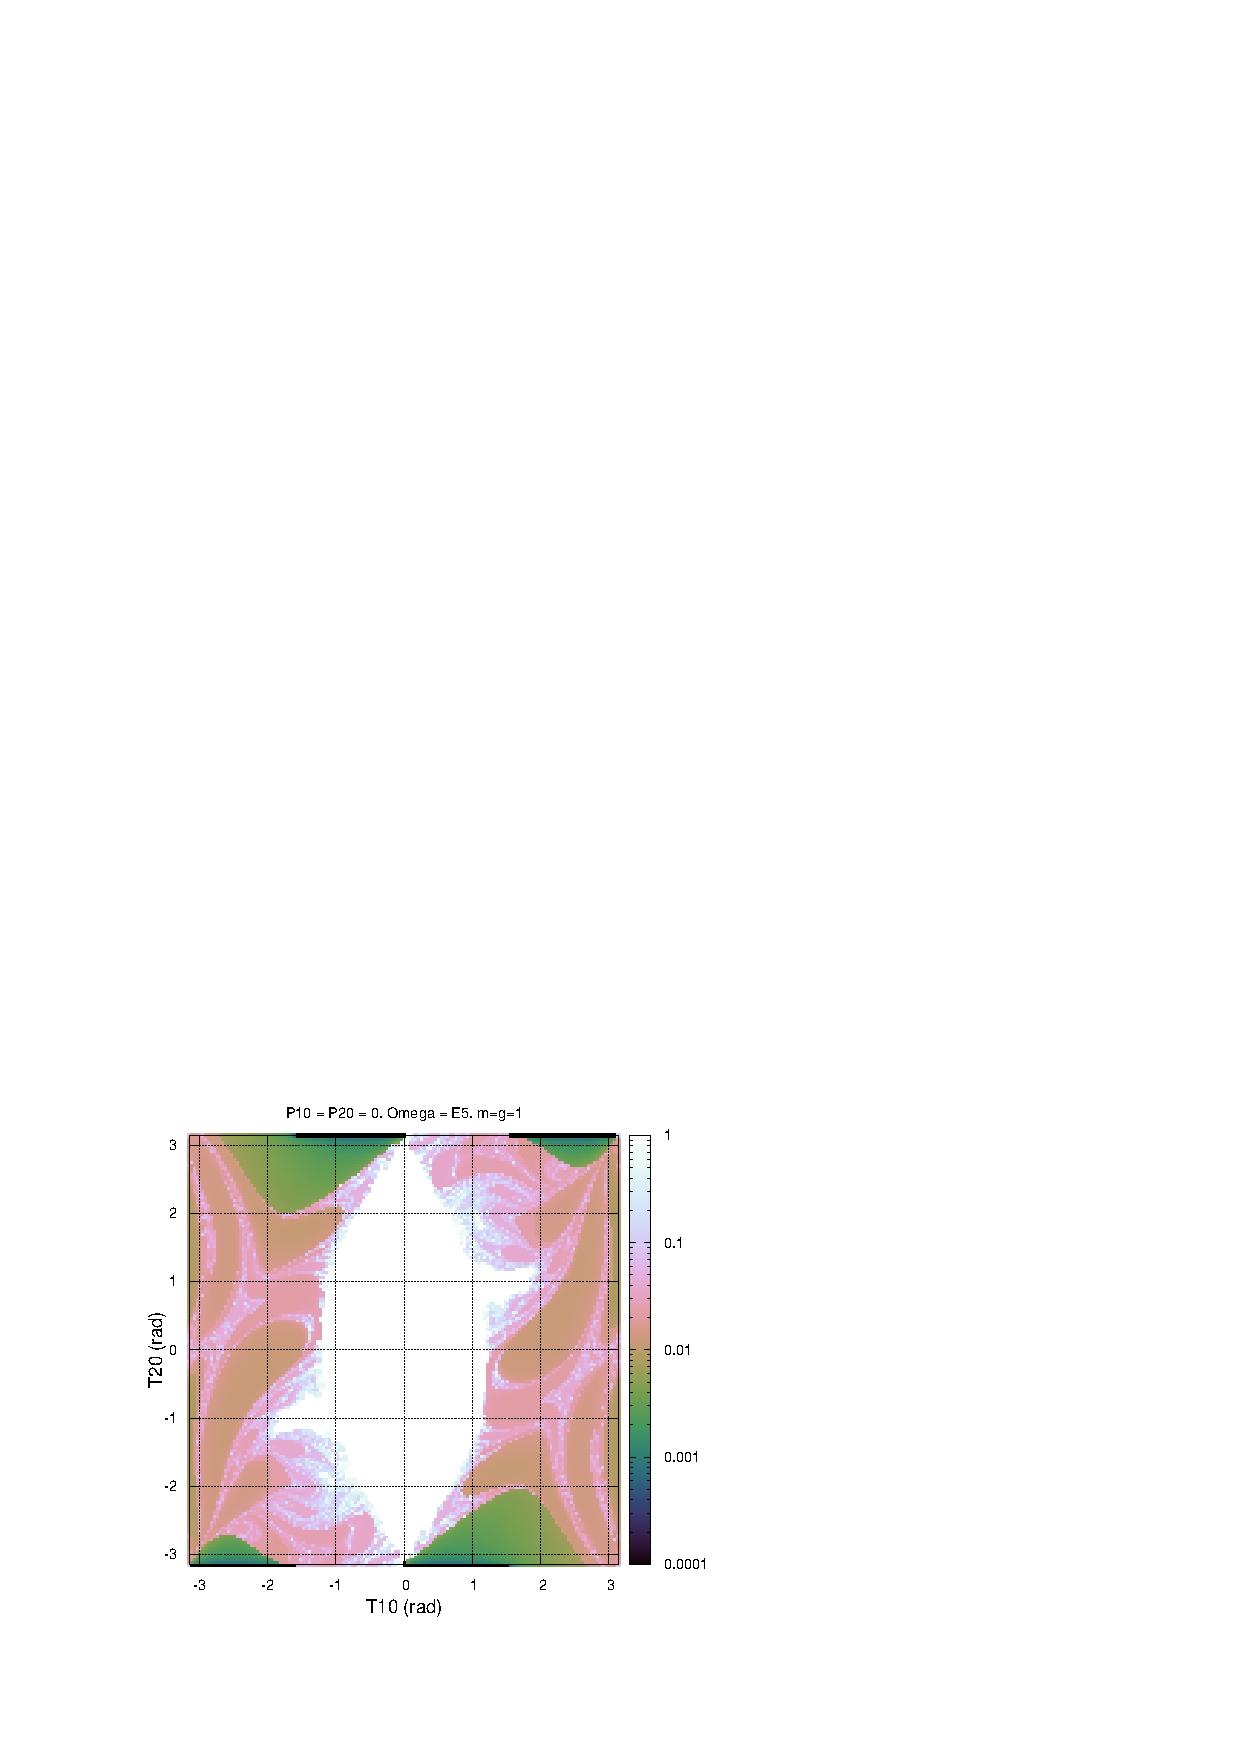
\includegraphics[scale=1.8]{Condiciones_Iniciales.pdf}
\caption{Dependencia del tiempo crítico ($t_c$) en función de los ángulos iniciales $\theta_{1,0}$ (T10) y $\theta_{2,0}$ (T20) para valores $P_{1,0} = P_{2,0} = 0$, $\omega^2 = 10^5$, $g=1$ y $m=1$.}\label{Fig-Caos}
\end{figure}
Las ecuaciones de movimiento del péndulo doble son: 
\begin{eqnarray*}
\dot{\theta_1} &=& \dfrac{6}{m\,l^2}\,\dfrac{2\,p_1 -3\,p_2\,\cos(\theta_1-\theta_2)}{16 - 9\,\cos^2(\theta_1-\theta_2)} \\
\dot{\theta_2} &=& \dfrac{6}{m\,l^2}\,\dfrac{8\,p_1 -3\,p_1\,\cos(\theta_1-\theta_2)}{16 - 9\,\cos^2(\theta_1-\theta_2)} \\
\dot{p_1} &=& -\dfrac{1}{2}\,m\,l^2\left( \dot{\theta_1}\,\dot{\theta_2}\,\sin(\theta_1-\theta_2) + 3\,\dfrac{g}{l}\,\sin(\theta_1)\right)\\
\dot{p_2} &=& -\dfrac{1}{2}\,m\,l^2\left(-\dot{\theta_1}\,\dot{\theta_2}\,\sin(\theta_1-\theta_2) + \dfrac{g}{l}\,\sin(\theta_1)\right).
\end{eqnarray*}
Para unas condiciones iniciales de $\theta_1$, $\theta_2$, $p_1$ y $p_2$ se resuelven mediante el método de Runge-Kutta. 
\\ \\
Se inicia el documento con la Figura \ref{Fig-Caos} para probar que el código funciona correctamente puesto que es una imagen amplicamente reportada en la literatura. 
\section*{0. Error}
Se define el error relativo en el presente documento como la diferencia relativa de la función ($\theta_1$, $\theta_2$, $p_1$ o $p_2$) en un tiempo $t=10$ con  un número determinado de puntos $N_i$ respecto al valor de la función para $t=10$ con un número de puntos $N_{i-1}$. En la Figura \ref{Fig-ErrorRelativo} se muestra el error relativo para cada una de las funciones de interés de acuerdo al número de puntos $N$. 
\\ \\
De acuerdo al comportamiento de la Figura \ref{Fig-ErrorRelativo}, se escoge como número de puntos, en todos los casos, $N = 10^4$. 
\begin{figure}
\centering 
\includegraphics[scale=1]{Graph_Harmonic_Oscillator.pdf}
\caption{Dependencia del error relativo en función del número de puntos $N$ para cada una de las funciones de interés del péndulo doble ($\theta_1$, $\theta_2$, $p_1$ o $p_2$) para $t=10$. Las constantes utilizadas fueron $m=1$, $g=1$, $l=1$, $\theta_{1,0} = \dfrac{\pi}{10}$, $\theta_{2,0} = \dfrac{\pi}{4}$, $p_{1,0} = 1$ y $p_{2,0} = 0$.}\label{Fig-ErrorRelativo}
\end{figure}
\section*{1. Espacio fase $t_c$ vs. $\omega^2$ para $\theta_{1,0} = \theta_{2,0}= \dfrac{\pi}{2}$ y $p_{1,0} = p_{2,0}=0$.}
El tiempo crítico se asume como aquel tiempo para el cual $|\theta_2| >\pi$. La Figura \ref{PhaseSpace1D} muestra el comportamiento del tiempo crítico en función de la frecuencia $\omega^2 = \dfrac{g}{l}$ (el valor de $g$ es siempre fijo, $g=1$) para condiciones iniciales de $\theta_{1,0} = \theta_{2,0} = \dfrac{\pi}{2}$  y $p_{1,0} = p_{2,0} = 0$. 
\begin{figure}
\centering
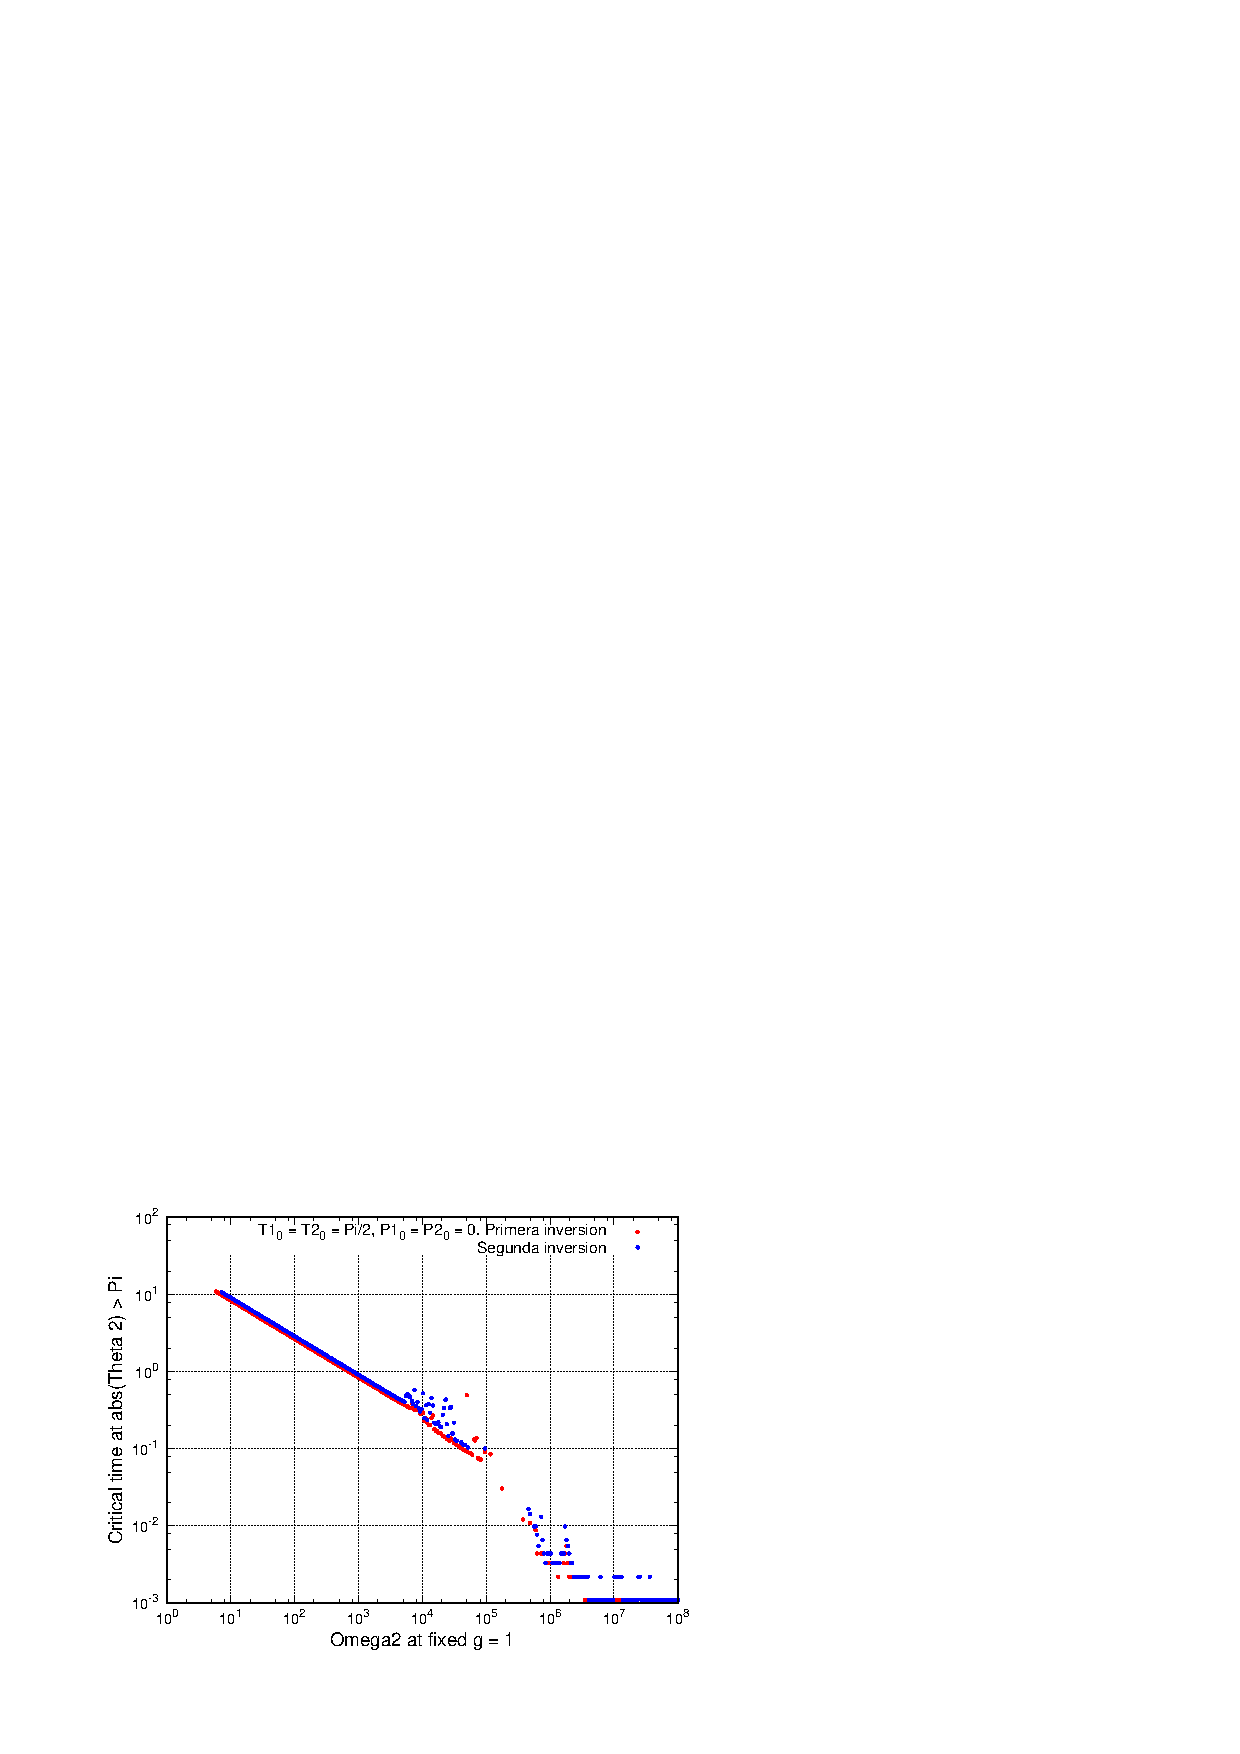
\includegraphics[scale=1]{Grafica_TCritico_L.pdf}
\caption{$t_c$ vs. $\omega^2$. En la figura se omite los valores de $t_c$ para $\omega^2 <$10 debido a que presenta un comportamiento similar al que se ilustra en el intervalo $10^1 < \omega^2 < 10^3$.}\label{PhaseSpace1D}
\end{figure}
\section*{2. Espacio fase $t_c$ vs. $\omega^2$ vs. $\theta_{1,0} = \theta_{2,0}$ para $p_{1,0} = p_{2,0}=0$.}
\begin{figure}
\centering
\includegraphics[scale=0.45]{2DPhaseSpace_1.png}
\caption{Dependencia del tiempo crítico, $t_c$, en función de $\omega^2$ y el ángulo inicial $\theta_{1,0} = \theta_{2,0}$ en un rango de frecuencias entre $1<\omega^2<10^8$.}\label{PhaseSpace2D-1}
\end{figure}
\begin{figure}
\centering
\includegraphics[scale=0.45]{2DPhaseSpace_2.png}
\caption{Dependencia del tiempo crítico, $t_c$, en función de $\omega^2$ y el ángulo inicial $\theta_{1,0} = \theta_{2,0}$ en un rango de frecuencias entre $10^5<\omega^2<10^{10}$. Nótese los recuadros, en donde se observa que para ciertas frecuencias y valores iniciales del angulo, el valor de $t_c$ no es continuo.}\label{PhaseSpace2D-2}
\end{figure}
En las Figuras \ref{PhaseSpace2D-1} y \ref{PhaseSpace2D-2} se muestran el comportamiento de $t_c$ en función de $\omega^2$ y de los ángulos iniciales, $\theta_{1,0} = \theta_{2,0}$. En la Figura \ref{PhaseSpace2D-2} se encierran ciertas zonas que presentan un comportamiento anómalo, similar al que se presenta para valores grandes de $\omega^2$ en la Figura \ref{PhaseSpace1D}.
\section*{3. Espacio fase $t_c$ vs. $\omega^2$ vs. $\theta_{1,0} = \theta_{2,0}$ variando $p_{1,0} = p_{2,0}$.} 
La dependencia del tiempo crítico en función de los momentos iniciales presenta algunos problemas debido a que, dado que las variaciones de $t_c$ se presenta para $\omega^2 > 10^5 $ (ver Figura \ref{PhaseSpace1D}), los tiempos críticos se vuelven pequeños ($\sim 10^{-6}$), esta es la razón por la cual los intervalos para $\omega^2$ en la Figura \ref{Fig-3DPhaseSpace} son del orden de $10^1 < \omega^2 < 10^4$. 
\\
\\
En la Figura \ref{Fig-3DPhaseSpace} se puede ver que, \textit{en los intervalos analizados} de $\omega^2$ y $\theta_{1,0} = \theta_{2,0}$, la variación de $t_c$ es suave (no caos). 
\begin{figure}
\centering 
\includegraphics[scale=0.8]{P1.pdf}
\includegraphics[scale=0.8]{P-1.pdf}
\includegraphics[scale=0.8]{PE-4.pdf}
\caption{Dependencia del tiempo crítico en función de $\omega^2$ y $\theta_{1,0} = \theta_{2,0}$ para diferentes valores de $p_{1,0} = p_{2,0} = -1, 1, 10^{-4}$.}\label{Fig-3DPhaseSpace}
\end{figure}
\section*{4. Trayectorias}
El análisis de las trayectorias se realiza para tres casos: ángulos pequeños, ángulos iniciales de $\dfrac{\pi}{2}$ y ángulos intermedios. 
\subsection*{4.1 Caso de ángulos pequeños: $\theta_{1,0} = \theta_{2,0} = \dfrac{\pi}{10}$ y $p_{1,0} = p_{2,0} = 0$}
Dado que se trata de ángulos pequeños, se encuentra un comportamiento similar a osciladores armónicos no acoplados. Las trayectorias y dependencias temporales se muestra en la Figura \ref{Fig-AngulosPeque}.
\begin{figure}
\centering
\includegraphics[scale=0.9]{SGrafica_Theta_Tiempo.pdf}
\includegraphics[scale=0.9]{SGrafica_P_Tiempo.pdf}
\includegraphics[scale=0.9]{SGrafica_EspacioFase.pdf}
\includegraphics[scale=0.9]{SGrafica_Trayectoria.pdf}
\caption{Resultado para \textbf{ángulos pequeños}. $p$ y $\theta$ en función del tiempo, espacio fase, y trayectoria para $0<t<20$}\label{Fig-AngulosPeque}
\end{figure}
\subsection*{4.2 Caso ángulos ``grandes'': $\theta_{1,0} = \theta_{2,0} = \dfrac{\pi}{2}$ y $p_{1,0} = p_{2,0} = 0$}
Las trayectorias y dependencias temporales se muestra en la Figura \ref{Fig-AngulosGrandes}. Las diferencias en los resultados para ángulos ``grandes'' son evidentes al compararse con los resultados de la Figura \ref{Fig-AngulosPeque}.
\begin{figure}
\centering
\includegraphics[scale=0.9]{BGrafica_Theta_Tiempo.pdf}
\includegraphics[scale=0.9]{BGrafica_P_Tiempo.pdf}
\includegraphics[scale=0.9]{BGrafica_EspacioFase.pdf}
\includegraphics[scale=0.9]{BGrafica_Trayectoria.pdf}
\caption{Resultado para \textbf{ángulos grandes}. $p$ y $\theta$ en función del tiempo, espacio fase, y trayectoria para $0<t<7$}\label{Fig-AngulosGrandes}.
\end{figure}

\subsection*{4.3 Caso ángulos intermedios: $\theta_{1,0} = \dfrac{\pi}{2}$, $\theta_{2,0} = \dfrac{\pi}{10}$, $p_{1,0} = -1$ y $p_{2,0} = 1$.}
Para las condiciones iniciales como las descritas anteriormente, es imposible preveer el comportamiento del péndulo doble. Los resultados se muestran en la Figura \ref{Fig-AngulosInter}.
\begin{figure}
\centering
\includegraphics[scale=0.9]{MGrafica_Theta_Tiempo.pdf}
\includegraphics[scale=0.9]{MGrafica_P_Tiempo.pdf}
\includegraphics[scale=0.9]{MGrafica_EspacioFase.pdf}
\includegraphics[scale=0.9]{MGrafica_Trayectoria.pdf}
\caption{Resultado para \textbf{ángulos intermedios}. $p$ y $\theta$ en función del tiempo, espacio fase, y trayectoria para $0<t<15$}\label{Fig-AngulosInter}.
\end{figure}
\section*{5. Segunda inversión de masa 2, $t_{c,2}$}
La segunda inversión se define como el tiempo para el cuál el ángulo de la  segunda partícula es $|\theta_2| > 3\pi$. Tal como se muestra en la Figura \ref{Fig-SegInversion}, los resultados para la segunda inversión son similares a los resultados para la primera inversión cuando la frencuencia es menor a $\omega^2 \sim 10^4$, una vez superado este límite, el comportamiento parecen no estar relacioandos.  
\begin{figure}
\centering
\includegraphics[scale=1.5]{2Grafica_TCritico_L.pdf}
\caption{Dependencia del tiempo crítico ($t_c$) para la primera y segunda inversión en función de los ángulos iniciales $\theta_{1,0}$ (T10) y $\theta_{2,0}$ (T20) para valores $P_{1,0} = P_{2,0} = 0$, $\omega^2 = 10^5$, $g=1$ y $m=1$.}\label{Fig-SegInversion}.
\end{figure}

\end{document}